\section{Results}
\subsection{Historical reconstruction and original model comparison}\label{sec:historical-loss}
The historical audit preserved original results and checked 1720 physical prediction files: 1240 earlier files by integrity checks and 480 compact-model files through recomputation. The 337120 physical metric rows exclude the extra 23520 V2-labeled alias rows. In the reproduced original comparison, thirty trained final states matched the archived reference states; an aggregate MASE discrepancy of $4.66\times10^{-10}$ was retained as numerical summary precision rather than interpreted as retraining improvement. Earlier pilot documents included a different partition, but the analysis here uses the actually executed 70/10/20 version.

Table~\ref{tab:historical-main} reports the six positive-loss conditions for the 28-service cohort. E5 has CPU MASE1.002387 versus E0's 0.992620, and memory MASE1.121358 versus 1.135901. Its mask-paired percentage changes are therefore unfavorable for CPU ($-0.984\%$ reduction) and favorable for memory ($1.280\%$). GRU with calls has the lowest displayed historical CPU MASE, 0.939410; this local result does not establish general graph superiority. Historical GinAR CPU MASE is 280825.103210, an extreme retained result of this implementation and budget. Verification did not justify discarding it or equating it with the published method's expected behavior.

\begin{table*}[!t]
\caption{Historical six-positive-loss means, source28, three neural seeds and twenty masks. Absolute CPU errors retain publisher scale and memory errors are bytes. V2 is a selected alias, not an additional fit. These values must not be mixed with destination32 errors.}\label{tab:historical-main}
\centering\footnotesize
\FitTable{\begin{tabular}{lrrrrrr}
\toprule
Model & CPU MASE & CPU MAE & CPU RMSE & Mem. MASE & Mem. MAE & Mem. RMSE \\
\midrule
persistencia & 1.07741 & 0.000300957 & 0.000505471 & 1.31287 & 1.30725e+06 & 2.01898e+06 \\
E0 & 0.99262 & 0.000302127 & 0.000456189 & 1.1359 & 1.10867e+06 & 1.694e+06 \\
E1 & 1.02275 & 0.000307441 & 0.000457202 & 1.1359 & 1.10867e+06 & 1.694e+06 \\
E2 & 1.02163 & 0.000305333 & 0.000453692 & 1.12503 & 1.09644e+06 & 1.6773e+06 \\
E3 & 1.00514 & 0.000304111 & 0.000455915 & 1.1345 & 1.10712e+06 & 1.69482e+06 \\
E4 & 0.98954 & 0.000301872 & 0.000456377 & 1.13528 & 1.10705e+06 & 1.69286e+06 \\
E5 & 1.00239 & 0.000305151 & 0.000455849 & 1.12136 & 1.0933e+06 & 1.67625e+06 \\
C0 & 1.02163 & 0.000305333 & 0.000453692 & 1.1359 & 1.10867e+06 & 1.694e+06 \\
C1 & 1.02095 & 0.000305271 & 0.000453709 & 1.1351 & 1.10785e+06 & 1.69341e+06 \\
C2 & 1.02151 & 0.000305326 & 0.000453707 & 1.13576 & 1.10848e+06 & 1.69381e+06 \\
C3 & 1.02092 & 0.000305271 & 0.000453723 & 1.13522 & 1.10794e+06 & 1.69342e+06 \\
V2 & 1.02092 & 0.000305271 & 0.000453723 & 1.1351 & 1.10785e+06 & 1.69341e+06 \\
GRU\_propia & 0.955358 & 0.000279717 & 0.0004371 & 1.16785 & 1.15154e+06 & 1.76786e+06 \\
GRU\_llamadas & 0.93941 & 0.000274958 & 0.000430716 & 1.19984 & 1.18269e+06 & 1.81389e+06 \\
BiTGraph\_codigo\_autor & 1.00373 & 0.000282931 & 0.000428389 & 1.21558 & 1.18535e+06 & 1.79317e+06 \\
GinAR & 280825 & 63.2538 & 1254.57 & 2.5045 & 2.27786e+06 & 4.49626e+06 \\
\bottomrule
\end{tabular}}
\end{table*}

Within E0--E5, E2's exponential component improves mean memory MASE to 1.125032 but worsens CPU to 1.021630. E4 gives the lowest CPU MASE among these six variants, 0.989540, while its memory MASE is 1.135284. E1 and E3 do not produce simultaneous resource gains. E5's combination is thus not a monotonic accumulation of improvements. The added memory benefit relative to E2 is a paired reduction of approximately 0.327\%, with more parameters and measured inference cost. These are independently selected configurations, so component names do not by themselves identify causal contributions.

\subsection{Compact C families, V2 and historical uncertainty}\label{sec:historical-compact}
C0--C3 reduce descriptor dimensionality without collapsing the two value heads. Their historical CPU MASE values are 1.021630, 1.020946, 1.021505 and 1.020919; memory values are 1.135901, 1.135097, 1.135755 and 1.135218. V2 selects C3/EMA0.7 for CPU and C1/MA25 for memory, with mean validation MASE0.911214 and 0.998329, respectively. The resulting test MASE is 1.020919/1.135097, with paired reductions of $-2.851\%$/$0.071\%$ against E0. Against E5 the reductions are $-1.849\%$/$-1.225\%$. Compactness therefore did not preserve E5's historical memory gain or improve both resources over E0.

The narrow mask-only E5 difference intervals are $[-0.010137,\allowbreak -0.009395]$ for CPU and $[0.014296,\allowbreak 0.014793]$ for memory. Crossing seed and mask resampling widens the CPU interval to $[-0.028165,\allowbreak 0.026164]$. The corresponding memory interval is $[-0.002967,\allowbreak 0.024027]$. Both include zero. One of three seed means favors E5 on CPU and two of three on memory. Although all 28 memory service means favor E5 after averaging other factors, those services are connected and share the same trace; this is not a binomial sample of infrastructures. Historical uncertainty therefore supports an observed memory advantage conditional on fits, with substantial initialization sensitivity.

Fig.~\ref{fig:historical} puts the historical rank and the extreme GinAR result on readable resource-specific axes. The historical displayed E0/E2/E4/E5/V2 curves rise across 0,10,20 and40\% loss under both original patterns for both resources. This yields twenty displayed increasing curves, not a theorem over every comparator or individual series. Historical CUDA B128 timing further shows why compression alone is insufficient: CPU-target E0/E5/V2 p50 values are 0.284/0.814/0.691 ms, and memory-target values 0.287/0.801/0.416 ms. V2 uses 28 CPU and27 memory parameters versus E5's74, but CPU V2 remains slower than E0. These ten-warmup eager measurements are not pooled with the later twenty-warmup B1 results.

\begin{figure*}[!t]\centering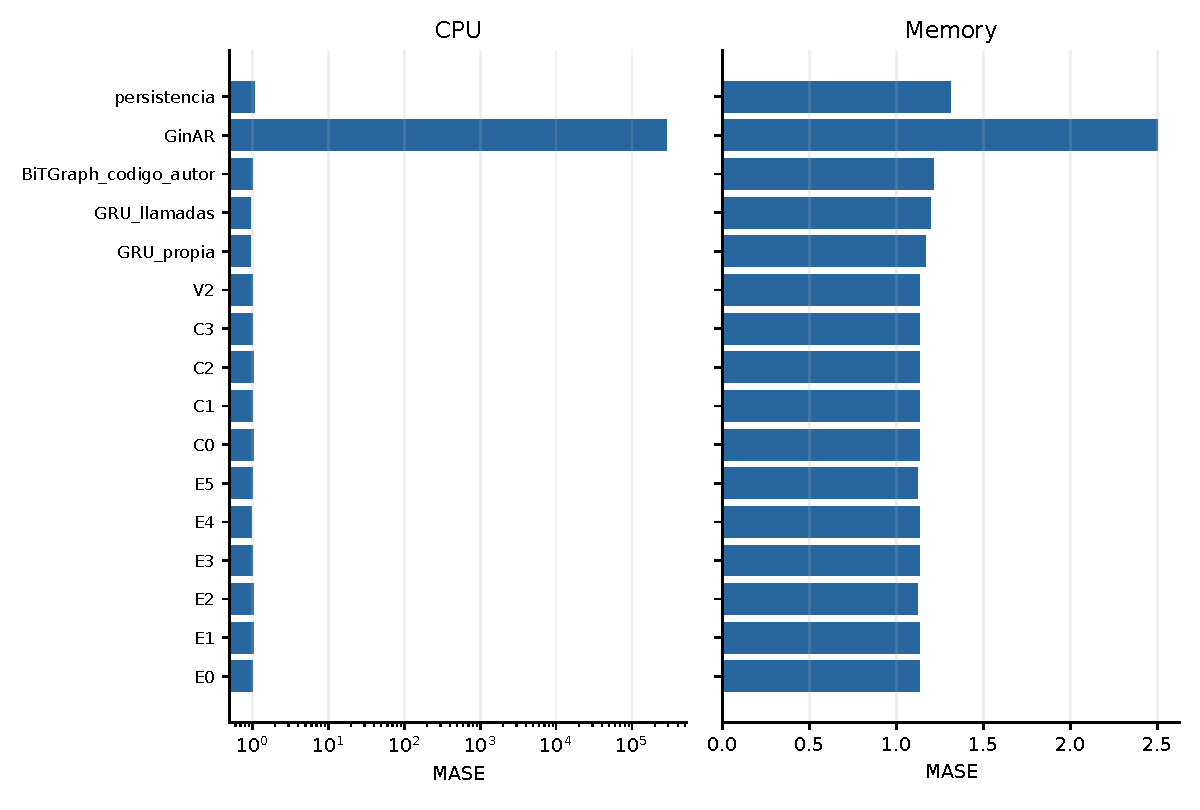
\includegraphics[width=0.82\textwidth]{figuras/historico.pdf}
\caption{Historical MASE under six positive-loss conditions. Logarithmic CPU scale preserves GinAR's extreme local value. Memory uses a linear scale. These are source28 results, not the destination comparison.}\label{fig:historical}
\end{figure*}
\begin{figure*}[!t]\centering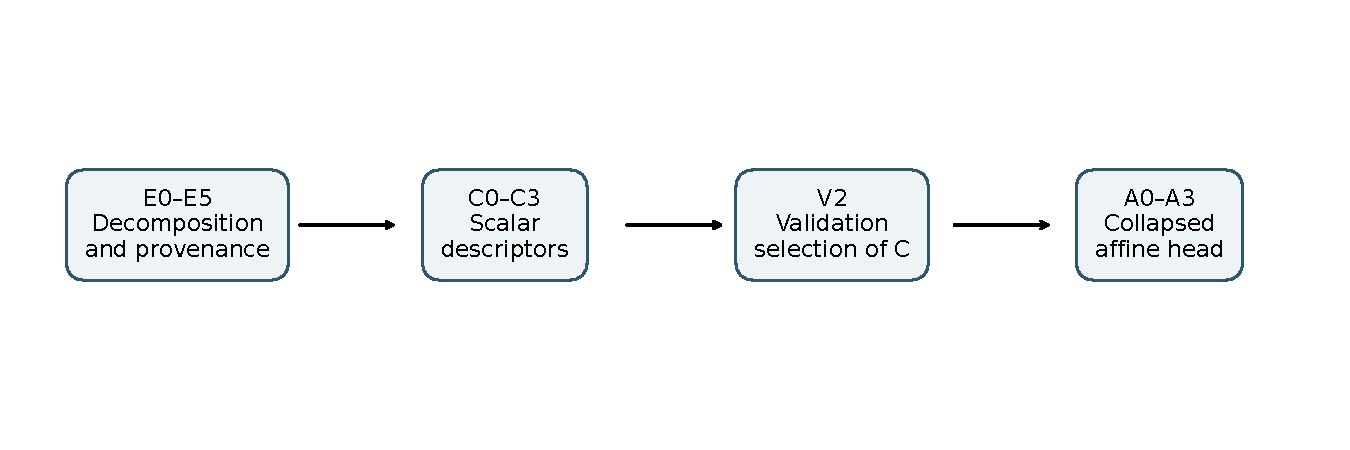
\includegraphics[width=0.91\textwidth]{figuras/evolucion.pdf}
\caption{Experimental progression: E changes decomposition or full descriptors; C retains two value heads with scalar descriptors; V2 selects existing C fits; A collapses the fixed affine value map. Arrows describe study order, not guaranteed accuracy gains.}\label{fig:evolution}
\end{figure*}
